\documentclass[border=5pt]{standalone}
\usepackage[T1]{fontenc}
\usepackage{lmodern,amsmath,amssymb,tikz}
\usetikzlibrary{arrows.meta,decorations.markings,calc,backgrounds}
\definecolor{branch}{RGB}{195,80,15}
\definecolor{branchB}{RGB}{18,125,105}
\definecolor{direct}{RGB}{37,82,156}
\definecolor{merged}{RGB}{109,57,133}
\definecolor{spoke}{RGB}{95,95,102}
\definecolor{srcgreen}{RGB}{22,120,55}
\tikzset{
  v/.style={circle,fill=black,inner sep=1.55pt},
  ins/.style={rectangle,draw=black,fill=white,line width=0.65pt,minimum size=4.6pt,inner sep=0pt},
  res/.style={line width=0.78pt,postaction={decorate},decoration={
    markings,
    mark=at position 0.48 with {\draw[line width=0.72pt,fill=white] (-0.27,-0.105) rectangle (0.27,0.105);},
    mark=at position 0.82 with {\arrow{Stealth[length=1.35mm,width=1.05mm]}}
  }},
  resns/.style={line width=0.78pt,postaction={decorate},decoration={
    markings,
    mark=at position 0.50 with {\draw[line width=0.72pt,fill=white] (-0.25,-0.10) rectangle (0.25,0.10);}
  }},
  source/.style={-{Stealth[length=1.55mm,width=1.15mm]},line width=0.75pt},
  reduce/.style={-{Stealth[length=2.0mm,width=1.45mm]},line width=0.9pt},
  lbl/.style={fill=white,inner sep=1.1pt}
}

\begin{document}
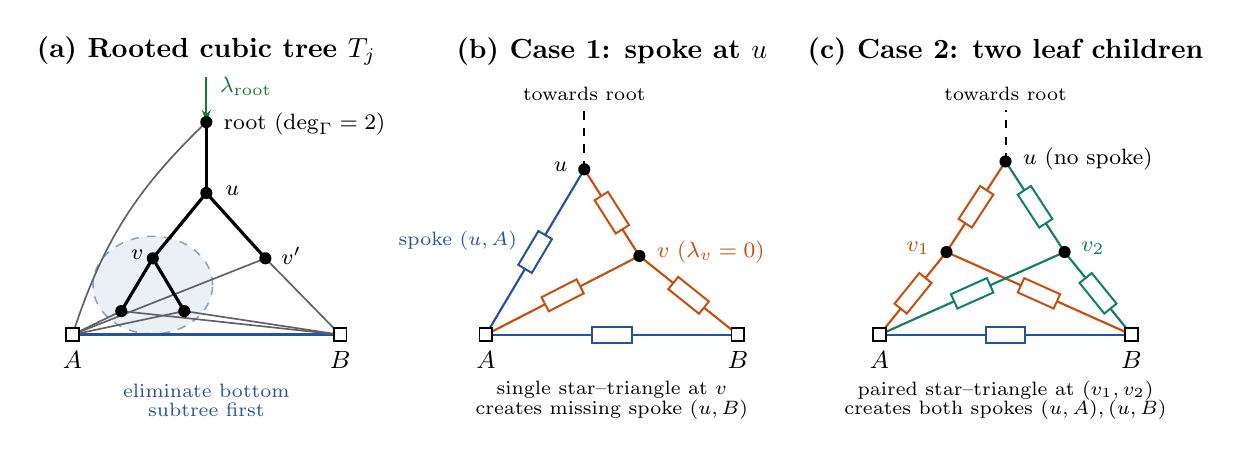
\begin{tikzpicture}[x=1cm,y=1cm,font=\small]

% Panel (a): Rooted cubic tree T_j
\begin{scope}[xshift=0cm]
  \node[font=\bfseries] at (1.9,3.95) {(a) Rooted cubic tree $T_j$};
  \coordinate (A) at (0.2,0.35);
  \coordinate (B) at (3.6,0.35);
  \coordinate (rt) at (1.9,3.05);
  \coordinate (u)  at (1.9,2.15);
  \coordinate (v)  at (1.22,1.32);
  \coordinate (vp) at (2.65,1.32);
  \coordinate (w1) at (0.82,0.65);
  \coordinate (w2) at (1.62,0.65);

  \begin{scope}[on background layer]
    \filldraw[fill=direct!9,draw=direct!55,dashed,line width=0.55pt] (1.22,0.98) ellipse (0.76cm and 0.62cm);
  \end{scope}

  \draw[direct,line width=1.05pt] (A)--(B);
  \draw[spoke,line width=0.6pt] (rt) to[bend right=14] (A);
  \draw[spoke,line width=0.6pt] (vp)--(A);
  \draw[spoke,line width=0.6pt] (vp)--(B);
  \draw[spoke,line width=0.6pt] (w1)--(A);
  \draw[spoke,line width=0.6pt] (w1)--(B);
  \draw[spoke,line width=0.6pt] (w2)--(A);
  \draw[spoke,line width=0.6pt] (w2)--(B);

  \draw[black,line width=1.15pt] (rt)--(u);
  \draw[black,line width=1.15pt] (u)--(v);
  \draw[black,line width=1.15pt] (u)--(vp);
  \draw[black,line width=1.15pt] (v)--(w1);
  \draw[black,line width=1.15pt] (v)--(w2);

  \draw[source,srcgreen] (1.9,3.62)--(rt);
  \node[srcgreen,right,font=\footnotesize] at (1.95,3.50) {$\lambda_{\mathrm{root}}$};
  \node[right,font=\footnotesize] at (2.0,3.03) {root ($\deg_\Gamma=2$)};
  \node[right,font=\footnotesize] at (2.02,2.18) {$u$};
  \node[left,font=\footnotesize,inner sep=1.5pt] at (1.16,1.36) {$v$};
  \node[right,font=\footnotesize] at (2.73,1.35) {$v'$};

  \node[ins,label=below:$A$] at (A) {};
  \node[ins,label=below:$B$] at (B) {};
  \foreach \p in {rt,u,v,vp,w1,w2}{\node[v] at (\p) {};}
  \node[direct,align=center,font=\scriptsize] at (1.9,-0.48) {eliminate bottom\\[-1pt]subtree first};
\end{scope}

% Panel (b): Case 1 - Parent u carries one spoke
\begin{scope}[xshift=5.15cm]
  \node[font=\bfseries] at (1.9,3.95) {(b) Case 1: spoke at $u$};
  \coordinate (A) at (0.3,0.35);
  \coordinate (B) at (3.5,0.35);
  \coordinate (u) at (1.55,2.45);
  \coordinate (v) at (2.25,1.35);

  \draw[dashed,line width=0.75pt] (u)--(1.55,3.20) node[above,font=\scriptsize]{towards root};
  \draw[resns,direct] (u)--(A);
  \draw[resns,direct] (A)--(B);
  \draw[resns,branch] (v)--(u);
  \draw[resns,branch] (v)--(A);
  \draw[resns,branch] (v)--(B);

  \node[direct,left,font=\scriptsize] at (0.82,1.55) {spoke $(u,A)$};
  \node[branch,right,font=\footnotesize] at (2.35,1.40) {$v$ ($\lambda_v=0$)};
  \node[left,font=\footnotesize] at (1.46,2.48) {$u$};

  \node[ins,label=below:$A$] at (A) {};
  \node[ins,label=below:$B$] at (B) {};
  \node[v] at (u) {};
  \node[v] at (v) {};
  \node[align=center,font=\scriptsize] at (1.9,-0.48) {single star--triangle at $v$\\[-1pt]creates missing spoke $(u,B)$};
\end{scope}

% Panel (c): Case 2 - Parent u has two leaf children
\begin{scope}[xshift=10.15cm]
  \node[font=\bfseries] at (1.9,3.95) {(c) Case 2: two leaf children};
  \coordinate (A) at (0.3,0.35);
  \coordinate (B) at (3.5,0.35);
  \coordinate (u)  at (1.9,2.55);
  \coordinate (v1) at (1.15,1.40);
  \coordinate (v2) at (2.65,1.40);

  \draw[dashed,line width=0.75pt] (u)--(1.9,3.20) node[above,font=\scriptsize]{towards root};
  \draw[resns,direct] (A)--(B);
  \draw[resns,branch] (v1)--(u);
  \draw[resns,branch] (v1)--(A);
  \draw[resns,branch] (v1)--(B);
  \draw[resns,branchB] (v2)--(u);
  \draw[resns,branchB] (v2)--(A);
  \draw[resns,branchB] (v2)--(B);

  \node[right,font=\footnotesize] at (2.0,2.58) {$u$ (no spoke)};
  \node[branch,left,font=\footnotesize] at (1.06,1.45) {$v_1$};
  \node[branchB,right,font=\footnotesize] at (2.74,1.45) {$v_2$};

  \node[ins,label=below:$A$] at (A) {};
  \node[ins,label=below:$B$] at (B) {};
  \node[v] at (u) {};
  \node[v] at (v1) {};
  \node[v] at (v2) {};
  \node[align=center,font=\scriptsize] at (1.9,-0.48) {paired star--triangle at $(v_1,v_2)$\\[-1pt]creates both spokes $(u,A),(u,B)$};
\end{scope}

\end{tikzpicture}
\end{document}
